\documentclass{article}

\usepackage[utf8]{inputenc}
\usepackage[french]{babel}
\usepackage{mathtools}
\usepackage{amssymb}
\usepackage{tikz}
\usetikzlibrary{matrix}
\usepackage{url}
\usepackage{enumitem}
\usepackage{multicol}
\usepackage{hyperref}

\hypersetup{
    colorlinks,
    citecolor=green,
    filecolor=blue,
    linkcolor=blue,
    urlcolor=blue
}

\usepackage{graphicx}
\newtheorem{theorem}{Théorème}
\newtheorem{lemma}{Lemme}
\newtheorem{corolaire}{Corollaire}
\newtheorem{proposition}{Proposition}
\newtheorem{definition}{Définition}
\newenvironment{proof}{{\sc Preuve:}}{~\hfill C.Q.F.D.}
\newenvironment{AMS}{}{}
\newenvironment{keywords}{}{}

\usepackage{epigraph}

% \epigraphsize{\small}% Default
\setlength\epigraphwidth{8cm}
\setlength\epigraphrule{0pt}

\usepackage{etoolbox}

\makeatletter
\patchcmd{\epigraph}{\@epitext{#1}}{\itshape\@epitext{#1}}{}{}
\makeatother

\title{Projet d'informatique semestre 3}
\author{Félix Desmaretz \& Maxime Flin}
\date{}

\begin{document}
\maketitle

Ce document est le compte-rendu du projet de \textbf{programmation orientée objet et interface graphique} réalisé en 2017 dans le cadre du troisième semestre de la licence d'informatique. Nous avons modélisé un jeu de l'oie et un jeu de numéri puis avons créé une interface graphique permettant de jouer en dehors de la console.
\tableofcontents
\newpage

\section{La modélisation}
Nous avons opté pour une modélisation basée sur un principe d'événements afin de rendre le jeu le plus modulable possible et d'exploiter au maximum les lambda expressions apparues dans Java8. 

Grâce à ce choix de modélisation, il suffit d'écrire de petits scripts pour modéliser un comportement. De plus, ces scripts peuvent parfaitement se superposer: cela rend très simple, par exemple, la création d'une case prison qui pose une question à chaque tour pouvant nous faire perdre des points.

De plus, l'utilisation de lambda expressions simplifie la lecture et la compréhension du code. Elle rend l'architecture du projet assez légère puisque pas encombrée par plein de classes héritées.

\subsection{Les événements}

Dans pour notre jeu, les événements que nous avons ajoutés sont les suivants:
\paragraph{Pour les joueurs}
\begin{enumerate}
\item Quand on commence son tour. C'est cet événement qui dit au joueur de lancer le dé et de déplacer ses pions.
\item Quand on finit son tour. Quand la joueur termine son tour on teste, par exemple, s'il a gagné
\item Quand on passe son tour. Quand le joueur ne peut pas jouer, il perd des points; décrémenter un compteur de tours à attendre...
\end{enumerate}

\paragraph{Pour les cases}
\begin{enumerate}
\item Quand un pion arrive sur la case. On peut, par exemple, vérifier si la case est déjà occupée, auquel cas on envoie le pion sur la case suivante ou précédente. On peut aussi poser une question au joueur dès qu'il arrive...
\item Quand un pion quitte la case. On peut changer l'état de la case d'~"occupé" à "libre".
\item Quand un pion reste sur la case. On peut décrémenter un nombre de tours à attendre.
\end{enumerate}

Toutes les actions du jeu sont basées sur l'implémentation de ces 6 événements qui sont déclenchés par la classe $Game$.

\subsection{Les classes de base}

\paragraph{La classe $Game$} est une classe abstraite représentant une partie. Il est important de noter qu'on considère ici, qu'au cours d'une exécution du programme, une seule partie peut être jouée. Ainsi la classe $Game$ demande d'implémenter les classes abstraites suivantes:

\begin{enumerate}
\item $setup$. Cette méthode a pour vocation de créer les cases du jeu et de placer tous les pions à leur position de départ.
\item $isEnd$. Cette méthode doit retourner vrai si le jeu est fini, faux sinon.
\end{enumerate}

Elle implémente l'interface $Iterable<Player>$ afin de pouvoir parcourir facilement la liste des joueurs inscrits et comprend une classe interne $State$ qui permet d'interagir avec le jeu. Cette dernière contient le cycle de joueur (càd l'ordre dans lequel les joueurs jouent) et permet d'influer dessus. $Game$ possède une instance statique de cette classe interne pour interagir avec elle à n'importe quel endroit dans le code.

Pour finir on trouve dans cette classe une instance de la classe $Board$, initialisé dans la méthode $start$, qui modélise la succession des tours.

\paragraph{Le $Board$} est une classe qui, au départ, implémentait l'interface $Iterable<Player>$ et qui permet modéliser la succession des tours. Elle a une classe interne Cycle qui représente le cycle de joueur, et qui implémentait au départ $Iterator<Player>$. La méthode $hasNext$ renvoie vrai tant qu'il y a des joueurs et la méthode $next$ renvoie le joueur suivant. 

Il est important de préciser qu'à l'origine, ces classes implémentaient des itérateurs: nous avons dû les modifier pour bien décrire le comportement de notre cycle de joueur. L'inconvénient étant qu'un simple itérateur ne permet pas d'implémenter la suppression d'un joueur. Nous avons trouvé que $ListIterator$ permettait de le faire. Elle demandait cependant d'écrire d'autres fonctionnalités qui ne nous étaient pas utiles; nous avons donc abandonné cet idée.

\paragraph{La classe $Player$} est une classe abstraite qui représente un joueur. Elle ne possède pas de méthode abstraites mais nous avons décidé de la faire quand même abstraite car elle ne possède pas de lien avec un Pion. Il est aisé de déduire que si le joueur n'a pas de pion il ne peut pas jouer.

Elle comprend néanmoins une classe interne qui implémente l'interface $ActionListener<Event>$ pour recevoir et déclencher des événements. Cette classe interne permet d'ajouter les actions à réaliser quand un joueur commence, finit ou passe son tour.

On trouve dans la classe $Player$ des classes internes qui représentent des comportements suffisamment "standard" pour l'avoir mis à cet endroit. Elles modélisent le déplacement d'un pion par un lancer de dés.

La classe $Player$ possède deux sous-classes: $GoosePlayer$ et $NumeriPlayer$ qui déterminent la relation entre le joueur et ses pions. Dans $GoosePlayer$ on trouve une fonction $getPawn$ qui renvoie un $Pawn$ et dans $NumeriPlayer$ une fonctions $pawns$ qui renvoie un tableau de $NumeriPawn$.

\paragraph{La classe $Pawn$} représente, comme son nom l'indique, un pion sur le plateau. C'est une classe assez vide. Elle possède deux méthodes $getLocation$ et $getPlayer$ qui renvoient respectivement l'instance de la case sur laquelle le pion se trouve et le joueur auquel il appartient. On trouve aussi la méthode $goToCell$ qui déplace le pion en prenant bien soin de déclencher les événements appropriés.

Dans le jeu de l'oie, on utilise directement la classe $Pawn$; dans le numeri, on utilise une sous classe $NumeriPawn$ qui possède un attribut entier constant correspondant au numéro porté par le pion.

\paragraph{La classe $Configuration$} a été ajoutée assez tardivement. Elle gère le paramétrage du jeu. Elle possède des classes internes décrivant les différents paramètres du jeu de l'oie et du numeri.

L'instance de cette classe est statique et constante. C'est à dire que, partout dans le projet, elle donne accès à la même instance de $Configuration$.

\begin{figure}
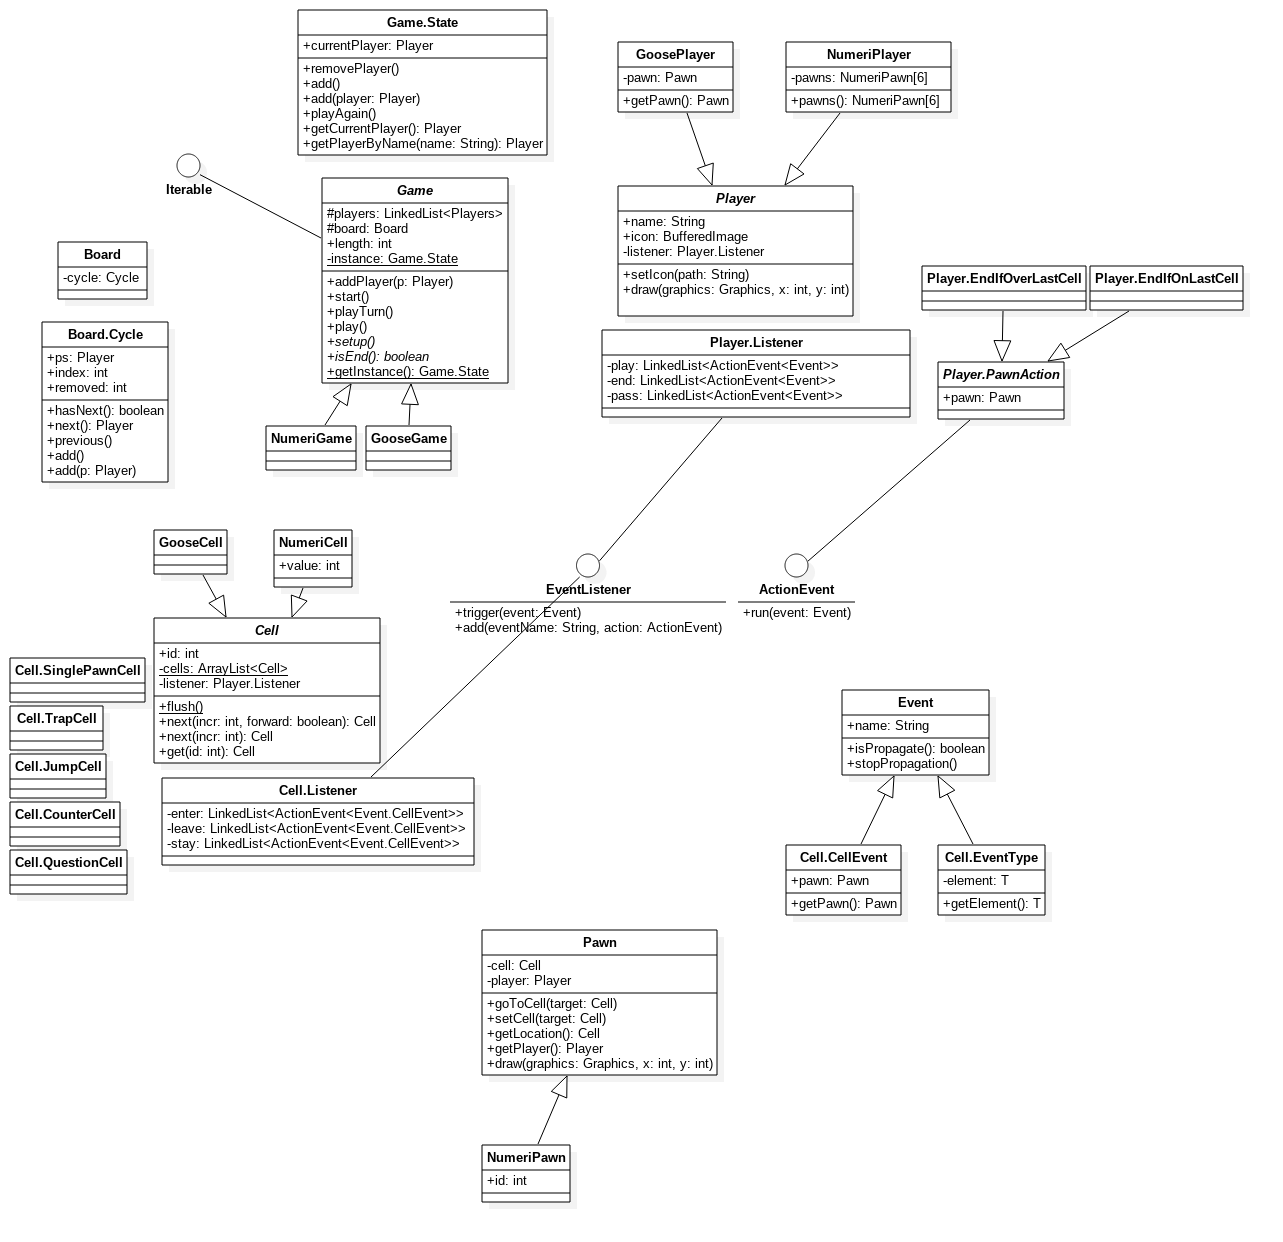
\includegraphics[width=\textwidth]{schema-uml.png}
\caption{
\textbf{Schéma du modèle.}
En carré les classes, en rond les interfaces, les champs précédés d'un $+$ sont publics, d'un $\#$ sont protected et d'un $-$ privés.}
\end{figure}

\section{L'interface graphique}
L'interface graphique fut de loin la partie la moins stimulante et la plus longue de ce projet, ne devenant intéressante que grâce à quelques fulgurances visant à lui donner un aspect plus personnel.

Dans le souci d'écrire un code bien organisé, propre et facilement modifiable, nous avons utilisé beaucoup de sous classes qui gèrent les aspects graphiques puis avons défini les interactions dans la classe englobante. Malgré tout, nous considérons cet aspect de notre projet n'est pas un franc succès car le code reste très confus et brouillon.

Le deuxième point qui demanderait à être retravaillé est le design des éléments natifs de java Swing: bien qu'il ait été modifié, il reste très sommaire (pour les boutons par exemple).

Pour finir, nos animations (planètes qui tournent sur elles-même, défilement du fond, météorites) sont très couteuses en performance. Il serait intéressant de retravailler la mise en place des $Thread$ pour n'en partager qu'un seul, qui devra sûrement être statique.

\section{Conclusion}
Pour conclure, nous pensons que ce projet aborde la modélisation du jeu sous un angle assez peu courant dans java compte tenu de la grande expressivité de la programmation orientée objet, bien que présent dans des langages plus récents comme $Javascript$ ou dans certains frameworks de développement de jeu vidéo, comme $Unity$.

Il y aurait, s'il fallait poursuivre, un travail de fond à faire sur l'interface graphique afin d'avoir quelque chose de vraiment accrocheur et performant. Nous pourrions ajouter sans trop de difficultés la possibilité de sauvegarder une partie, d'éditer complètement le plateau et de le partager avec ses amis. Le modèle étant fait en java, une version du jeu sous android est tout à fait envisageable (nous précisons bien envisageable, car nous doutons d'en avoir un jour envie).

\newpage
\nocite{*}

\bibliographystyle{plain}

\end{document}
